\documentclass[12pt]{extarticle}
%Some packages I commonly use.
\usepackage[portuguese]{babel}
\usepackage{graphicx}
\usepackage{framed}
\usepackage[normalem]{ulem}
\usepackage{amsmath}
\usepackage{amsthm}
\usepackage{amssymb}
\usepackage{amsfonts}
\usepackage{enumerate}
\usepackage[utf8]{inputenc}
\usepackage{float}
\usepackage{gensymb}
\usepackage[top=1 in,bottom=1in, left=1 in, right=1 in]{geometry}
\usepackage{multirow}
\usepackage{caption}
\usepackage{subcaption}
\usepackage[utf8]{inputenc}
\usepackage{tikz} 

%A bunch of definitions that make my life easier
\newcommand{\matlab}{{\sc Matlab} }
\newcommand{\cvec}[1]{{\mathbf #1}}
\newcommand{\rvec}[1]{\vec{\mathbf #1}}
\newcommand{\ihat}{\hat{\textbf{\i}}}
\newcommand{\jhat}{\hat{\textbf{\j}}}
\newcommand{\khat}{\hat{\textbf{k}}}
\newcommand{\minor}{{\rm minor}}
\newcommand{\trace}{{\rm trace}}
\newcommand{\spn}{{\rm Span}}
\newcommand{\rem}{{\rm rem}}
\newcommand{\ran}{{\rm range}}
\newcommand{\range}{{\rm range}}
\newcommand{\mdiv}{{\rm div}}
\newcommand{\proj}{{\rm proj}}
\newcommand{\R}{\mathbb{R}}
\newcommand{\N}{\mathbb{N}}
\newcommand{\Q}{\mathbb{Q}}
\newcommand{\Z}{\mathbb{Z}}
\newcommand{\<}{\langle}
\renewcommand{\>}{\rangle}
\renewcommand{\emptyset}{\varnothing}
\newcommand{\attn}[1]{\textbf{#1}}
\theoremstyle{definition}
\newtheorem{theorem}{Theorem}
\newtheorem{corollary}{Corollary}
\newtheorem*{definition}{Definition}
\newtheorem*{example}{Example}
\newtheorem*{note}{Note}
\newtheorem{exercise}{Exercise}
\newcommand{\bproof}{\bigskip {\bf Proof. }}
\newcommand{\eproof}{\hfill\qedsymbol}
\newcommand{\Disp}{\displaystyle}
\newcommand{\qe}{\hfill\(\bigtriangledown\)}
\setlength{\columnseprule}{1 pt}
\usepackage[utf8]{inputenc}

\usetikzlibrary{arrows,shapes,positioning}
\usetikzlibrary{decorations.markings}
\usetikzlibrary{angles}
\tikzstyle arrowstyle=[scale=1]
\tikzstyle directed=[postaction={decorate,decoration={markings,
    mark=at position .65 with {\arrow[arrowstyle]{stealth}}}}]
\tikzstyle reverse directed=[postaction={decorate,decoration={markings,
    mark=at position .65 with {\arrowreversed[arrowstyle]{stealth};}}}]

\title{Aula 17 - Espelhos}
\author{Felipe Salvador}
\date{Atualizado em \today}

\begin{document}

\maketitle

\section{Introdução}
Nessa aula, iremos estudar um dos objetos mais importantes em ótica e como ele altera o caminho que a luz faz: o espelho. A partir dele, iremos deduzir as relações principais para 2 tipos de espelho: o plano e o esférico.

\section{Espelho Plano}
O espelho plano é o tipo de espelho que não altera o formato, tamanho da imagem em relação ao objeto. É o espelho mais usado no dia a dia, presente em banheiros e lojas.

O que caracteriza um espelho plano é o seguinte: \textbf{O ângulo de incidência da luz em relação à normal é igual ao ângulo de reflexão da luz em relação à normal.}

\begin{figure}[H]
    \centering
    \begin{tikzpicture}

    % define coordinates
    \coordinate (O) at (0,0) ;
    \coordinate (A) at (0,4) ;
    \coordinate (B) at (0,-4) ;
    \coordinate (P) at (-2,2)
    
    % media

    % axis
    \draw[dash pattern=on5pt off3pt] (O) -- (A) ;
    \draw[black, ultra thick] (-4,0) -- (4,0);
    \draw[black, thick] (3.7,-0.2) -- +(0.2,0.2);
    \draw[black, thick] (3.5,-0.2) -- +(0.2,0.2);
    \draw[black, thick] (3.3,-0.2) -- +(0.2,0.2);

    % rays
    \draw[red,ultra thick,reverse directed] (O) -- (P);
    \draw[blue,directed,ultra thick] (O) -- (2,2);

    % angles
    \draw (0,2) arc (90:130:2.1);
    \draw (1.5,1.45) arc (50:90:2.3) ;
    \filldraw [black] (-2,2) circle (2pt);
    \filldraw [black] (2,2) circle (2pt);
    \node[] at (70:1.7)  {$\theta$};
    \node[] at (110:1.7)  {$\theta$};
    \node[] at (-2,2.5) {A};
    \node[] at (2,2.5) {B};
\end{tikzpicture}
    \caption{Esquema de reflexão da luz num espelho plano. Em vermelho, é o raio de luz incidindo e em azul é o raio de luz refletido pelo espelho. O tracejado cinza é a reta normal do espelho.}
    \label{fig:my_label}
\end{figure}

\subsection{Imagem de um objeto num espelho plano}

Quando colocamos um objeto a frente de um espelho, o comportamento do objeto é o seguinte:
\begin{figure}[H]
    \centering
    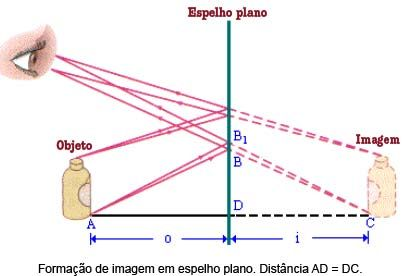
\includegraphics[width=0.6\textwidth]{plano_1.jpg}
    \caption{Esquema da formação de imagem de uma garrafa a frente de um espelho.}
    \label{fig:plano_1}
\end{figure}

A característica importante é que \textbf{a distância entre a imagem e o espelho (segmento DC) é a mesma entre o objeto e o espelho (segmento AD).} Essa é uma característica especial do espelho plano.

Uma outra questão interessante é sobre a forma das imagens num espelho plano. Quando colocamos um objeto que não é simétrico, a imagem no espelho vai aparentar um pouco diferente.

O fenômeno que acontece no espelho é chamado de \textbf{enantiomorfismo}, que é quando temos uma inversão da direita para a esquerda do objeto:

\begin{figure}[H]
    \centering
    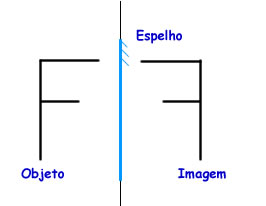
\includegraphics[width=0.5\textwidth]{enantiomorfismo.jpg}
    \caption{Esquema do enantiomorfismo da imagem num espelho.}
    \label{fig:enantiomorfismo}
\end{figure}
\subsection{Objeto ou espelho se movimentando}
Quando o objeto e o espelho não estão parados entre si, um efeito interessante acontece com a imagem do espelho: ela começa a se movimentar também.

Se um objeto começa a se mover com uma velocidade 'v' em relação ao espelho, a imagem também se move com velocidade 'v' em relação ao espelho, \textbf{só que no sentido contrário}.

\begin{figure}[H]
    \centering
    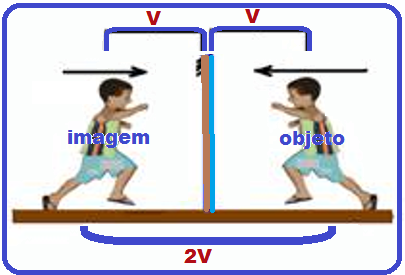
\includegraphics[width=0.5\textwidth]{objeto se movimentando.png}
    \caption{Esquema de objetos se movimentando a frente de um espelho.}
    \label{fig:mov_espelho}
\end{figure}

O mais interessante disso tudo é que, para o objeto, a imagem está se movimentando com a velocidade de '2v' em relação a você. 

\subsection{Associação de espelhos planos}

Quando colocamos 2 espelhos planos, em que entre eles forma-se um ângulo $\alpha$, e colocamos um objeto na frente desses espelhos, acontece a formação de múltiplas imagens, como na figura a seguir:
\begin{figure}[H]
    \centering
    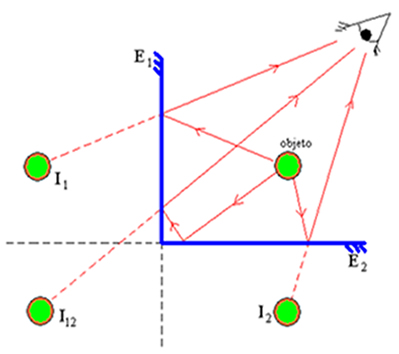
\includegraphics[width=0.5\textwidth]{associacao.jpg}
    \caption{Esquema de associação entre espelhos em que os espelhos, nesse caso, formam um ângulo de $\alpha=90^\circ$. Perceba que formou 3 imagens.}
    \label{fig:associacao}
\end{figure}

Há uma fórmula para achar o número de imagens formadas pela associação de 2 espelhos planos:
\begin{equation}
    N = \frac{360}{\alpha} -1
\end{equation}
\noindent em que $\alpha$ é o ângulo formado pelos 2 espelhos. Caso o resultado dê um número decimal, descarte os decimais e fique com a parte inteira.

\section{Espelhos esféricos}

Esse tipo de espelho é feito no formato de uma calota esférica (uma seção da superfície de uma esfera). Esses espelhos são construídos para o uso de espelhos de maquiagem, satélites, espelhos de saída de garagem, etc. Abaixo temos um esquema de um espelho esférico e como a luz se comporta na reflexão.
\begin{figure}[H]
    \centering
    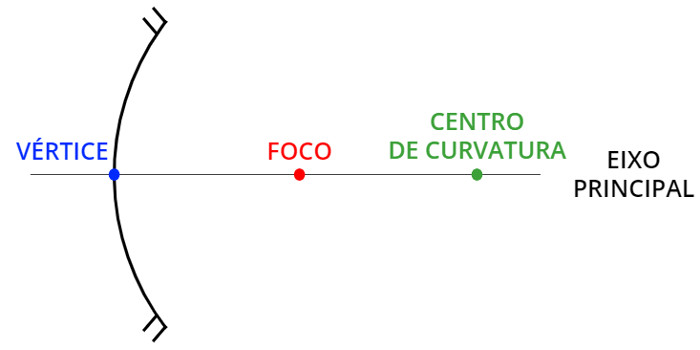
\includegraphics[width=0.5\textwidth]{esferico_1.jpg}
    \caption{Esquema de um espelho esférico.}
    \label{fig:esferico}
\end{figure}

Vamos entender o que cada um desses pontos significa:
\begin{itemize}
    \item O 'Eixo Principal' é a reta que passa no centro geométrico da esfera e vai até a borda do espelho;
    \item O 'Vértice' (V) é o ponto em que o eixo principal cruza o espelho;
    \item O 'Centro de Curvatura' (C) é o ponto que representa o centro da esfera a qual o espelho foi montado. A distância entre o Vértice e o Centro é o raio da esfera ou do espelho;
    \item O 'foco' é um ponto do espelho devido a 2 casos:
    
    1-) Quando o raio de luz chega ao espelho paralelo ao eixo principal, após a reflexão, o raio passa pelo foco.
    
    2-) Quando o raio de luz passa pelo foco antes da reflexão, após ela, o raio de luz sai paralelo ao eixo principal.
    
    Isso ficará claro nos exemplos a seguir.
\end{itemize}

Há 2 tipos de espelhos:
\begin{enumerate}
    \item \textbf{Espelho Côncavo} - é quando a luz reflete na parte interna da superfície da esfera. Após a reflexão, os raios de luz se concentram;
    \item \textbf{Espelho Convexo} - é quando a luz reflete na parte exterior da superfície da esfera. Após a reflexão, os raios de luz se distanciam um dos outros.
\end{enumerate}

\textbf{Uma questão importante é que, para um espelho convexo, o foco e o centro são VIRTUAIS, ou seja, eles estão 'atrás do espelho}

\begin{figure}[H]
    \centering
    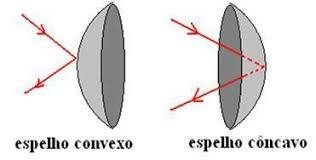
\includegraphics[width=0.5\textwidth]{concavo_convexo.jpg}
    \caption{Esquema dos espelhos côncavos e convexos}
    \label{fig:concavos-convexos}
\end{figure}

\subsection{Raios Notáveis}
Nessa seção, vamos estudar quais são os raios de luz mais importantes no estudo ótico. Ao todo, são 4 raios principais.
\begin{enumerate}
    \item \textbf{Vem paralelo ao eixo principal e sai passando pelo foco}
    \begin{figure}[H]
        \centering
        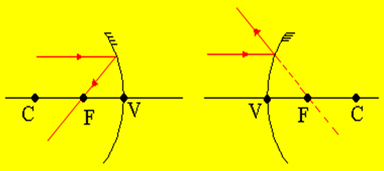
\includegraphics[width=0.5\textwidth]{raio_principal_1.jpg}
        \label{fig:raio_principal_1}
    \end{figure}
    
    \item \textbf{Vem pelo foco e sai passando eixo principal}
    \begin{figure}[H]
        \centering
        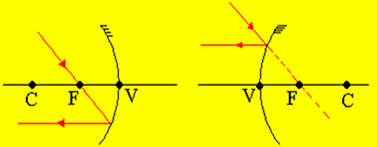
\includegraphics[width=0.5\textwidth]{raio_principal_2.jpg}
        \label{fig:raio_principal_2}
    \end{figure}
    
    \item \textbf{Vem pelo vértice e sai por ele (o ângulo de incidência é igual ao de reflexão)}
    \begin{figure}[H]
        \centering
        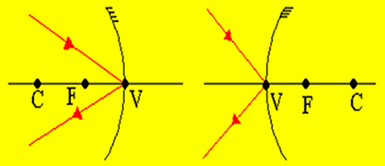
\includegraphics[width=0.5\textwidth]{raio_principal_3.jpg}
        \label{fig:raio_principal_3}
    \end{figure}
    
    \item \textbf{Vem pelo centro e volta pelo o mesmo caminho}
    \begin{figure}[H]
        \centering
        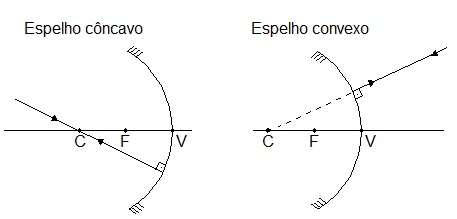
\includegraphics[width=0.6\textwidth]{raio_principal_4.jpg}
        \label{fig:raio_principal_4}
    \end{figure}
\end{enumerate}

\subsection{Determinação da Imagem}
Ao todo, a imagem se comporta de 5 maneira possíveis 5 para o Espelho côncavo e 1 maneira para o espelho convexo.

\subsubsection{Espelho côncavo}
\begin{enumerate}
    \item \textbf{Objeto atrás do centro}
    \begin{figure}[H]
        \centering
        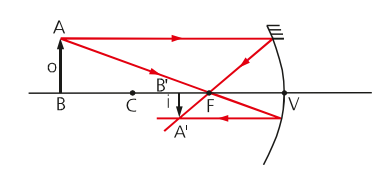
\includegraphics[width=0.5\textwidth]{concavo_caso_1.png}
        \label{fig:concavo_caso_1}
    \end{figure}
    Nesse caso, a imagem é \textbf{real (tá no mesmo lado do objeto), invertida (tá para baixo do eixo) e menor que o objeto.}
    
    \item \textbf{Objeto sobre o centro}
    \begin{figure}[H]
        \centering
        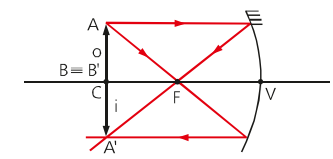
\includegraphics[width=0.5\textwidth]{concavo_caso_2.png}
        \label{fig:concavo_caso_2}
    \end{figure}
    Nesse caso, a imagem é \textbf{real (tá no mesmo lado do objeto), invertida (tá para baixo do eixo) e mesmo tamanho do que o objeto.}
    
    \item \textbf{Objeto entre o foco e o centro}
    \begin{figure}[H]
        \centering
        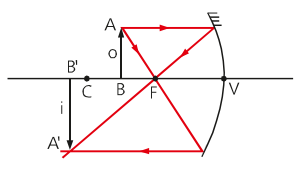
\includegraphics[width=0.5\textwidth]{concavo_caso_3.png}
        \label{fig:concavo_caso_3}
    \end{figure}
    Nesse caso, a imagem é \textbf{real (tá no mesmo lado do objeto), invertida (tá para baixo do eixo) e maior que o objeto.}
    
    \item \textbf{Objeto sobre o foco}
    \begin{figure}[H]
        \centering
        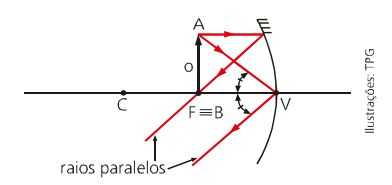
\includegraphics[width=0.5\textwidth]{concavo_caso_4.png}
        \label{fig:concavo_caso_4}
    \end{figure}
    Nesse caso, a imagem é \textbf{imprópria (não a formação de imagem ou a imagem se forma no infinito)}.
    
    \item \textbf{Objeto entre o foco e o vértice}
    \begin{figure}[H]
        \centering
        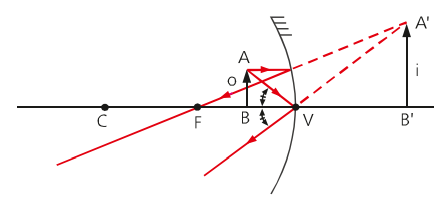
\includegraphics[width=0.5\textwidth]{concavo_caso_5.png}
        \label{fig:concavo_caso_5}
    \end{figure}
    Nesse caso, a imagem é \textbf{virtual (tá no outro lado do espelho), direita (tá para cima do eixo) e maior que o objeto.}
\end{enumerate}

\subsubsection{Espelho Convexo}
\begin{enumerate}
    \item \textbf{Caso Geral}
    \begin{figure}[H]
        \centering
        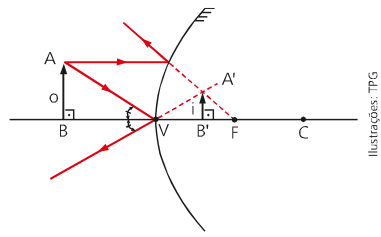
\includegraphics[width=0.5\textwidth]{convexo_caso.png}
        \label{fig:convexo_caso_geral}
    \end{figure}
    Nesse caso, a imagem é \textbf{virtual (tá no outro lado do espelho), direita (tá para cima do eixo) e menor.}
\end{enumerate}

\section{Equações Óticas}
Nessa parte, temos 2 equações importantes. A primeira é a chamada \textbf{Equação de Gauss:}
\begin{equation}
    \frac{1}{f} = \frac{1}{p} + \frac{1}{p'}
\end{equation}
\noindent em que 'f' é a distância focal (distância entre o foco e o vértice); 'p' é a distância entre o objeto e o vértice; "$p'$" é a distância entre a imagem e o foco. Abaixo está tudo descrito na imagem:
\begin{figure}[H]
    \centering
    \includegraphics[width=0.5\textwidth]{parâmetros.jpg}
    \caption{Esquema das quantidades importantes no estudo de espelhos}
    \label{fig:parametros}
\end{figure}

Questões importantes:
\begin{itemize}
    \item Caso o espelho seja côncavo, a distância focal é positiva $f>0$. Caso o espelho seja convexo, a distância focal é negativa $f<0$;
    \item Caso a imagem seja real (ou seja, esteja no mesmo lado do objeto), a distância p' é positiva: $p'>0$. Caso a imagem esteja virtual (ou seja, atrás do espelho), a distância p' é negativa: $p'<0$.
\end{itemize}

A outra equação que usamos é a \textbf{Equação do Aumento Linear}:
\begin{equation}
    A = \frac{i}{o} = \frac{-p'}{p} = \frac{f}{f-p}
\end{equation}
\noindent em que 'i' é o tamanho da imagem, 'o' é o tamanho do objeto, 'f' é a distância focal, 'p' é a distância entre o objeto e o vértice e "p'" é a distância entre a imagem e o vértice.

Caso o resultado seja negativo, isso significa que a imagem é invertida. Caso o resultado esteja entre $0<A<1$, significa que a imagem é menor que o objeto e, caso o resultado $A>1$, isso significa que a imagem é maior que o objeto.
\end{document}
